\chapter{Prototypische Implementierung}
\label{chap:impl}
Dieses Kapitel widmet sich der prototypischen Implementierung der im vorigen Kapitel vorgestellen Konzeption, die als Vorgabe in C++ entwickelt werden muss. Anhand des UML-Klassendiagrammes in \Fref[plain]{fig:uml} wird der grobe Aufbau gezeigt. Als nächster Punkt wird die Abstraktion des Netwerkes erklärt. Danach wird -- ausgehend von der Applikation -- die Implementierung des Publish/Subscribe-Systems erläutert. Angewandte Techniken wie \ac{tmp} oder \emph{policy based}-Design werden am Ende dieses Kapitels eingeführt. Sie werden benötigt um den zusätzlichen Verwaltungsaufwand zur Laufzeit durch geschickte Anwendung des zur Übersetzungszeit vorhandenen Wissens zu minimieren. Das nutzbare Wissen umfasst zum Beispiel die Typen der Events, die zur Optimierung ausgewählten Strategien und deren Besonderheiten.

\section{Implementierungsdetails}
\label{chap:impl_impl}

\begin{figure}[htbp]
\centering
\resizebox{\textwidth}{!}{%
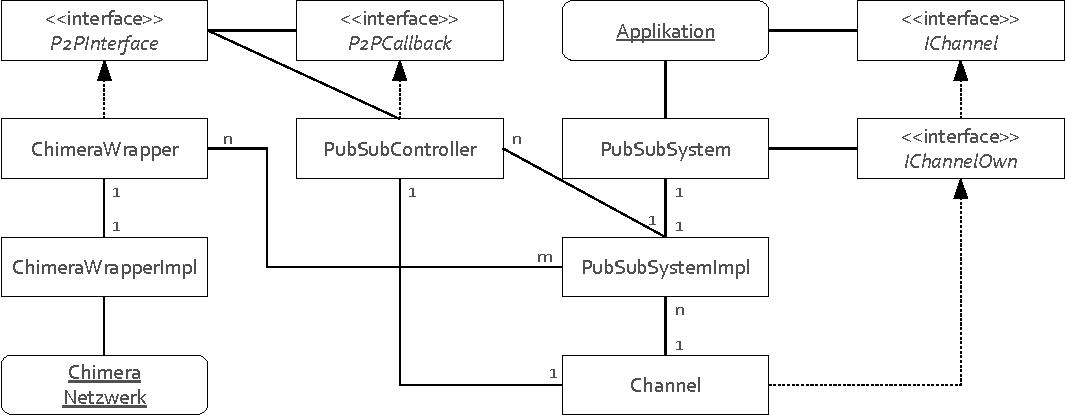
\includegraphics{grafics/uml.pdf}}
\caption{vereinfachtes Klassendiagramm des Frameworks}
\label{fig:uml}
\end{figure}

\emph{P2PInterface} ist eine abstrakte Basisklasse und repräsentiert die in \cite{Dabek2003Towards} beschrieben KBR-API. Aktuell wird diese vom \emph{ChimeraWrapper} implementiert, der über den \emph{ChimeraWrapperImpl} mit dem Netzwerk Chimera spricht. Hier wurde das ``PIMPL''-Pattern angewandt, mit dem die eigentliche Implementierung versteckt werden kann \cite{Alexandrescu2001Modern}.

Die \emph{Applikation} spricht mit dem \emph{PubSubSytem}, dessen Implementierung auch in einer eigenen Klasse ausgelagert ist. Die Applikation und das PubSubSystem kennen den \emph{Channel} nur über die abstrakte Basisklasse \emph{IChannel} beziehungsweise \emph{IChannelOwn}. Durch diese beiden Basisklassen wird die Komplexität der durch Policies optimierten Klasse Channel verdeckt. Die Klasse \emph{PubSubController} implementiert das Interface \emph{P2PCallback} und kann sich somit für die Callbacks des Netzwerkes registrieren. Weiterhin bietet diese Klasse die von Channel benötigte Funktionalität. PubSubSystemImpl kennt die Netzwerkwrapperklassen (in \Fref{fig:uml} ChimeraWrapper) und verbindet diese über den PubSubController mit dem Channel. Mit verschiedene Instanzen des PubSubControllers können somit auch verschiedene Netzwerke angesprochen werden und entsprechend der Optimierung für verschiedene Channel eingesetzt werden.

\subsection{Netzwerkabstraktion}
\begin{itemize*}
\item Abstrakte Basisklasse für Netzwerk
\item Abstrakte Basisklasse für Netzwerkupcalls
\item Wrapperklassen für jedes Netzwerk
\end{itemize*}


\subsection{PubSubabstraktion}
\begin{itemize*}
\item PubSubController spricht mit Netzwerk
\item PubSubSystem spricht mit Applikation und leitet Anfragen an Channel weiter
\item Channel nutzt Controller zum Netzwerkzugriff
\item $\rightarrow$ Möglichkeit verschiedene Netzwerke zu nutzen!
\end{itemize*}

\subsection{Channel}
The different optimization strategies for each dimension are implemented as policies encapsulating their behaviour. Each channel is therefore a template class with all dimensions as template parameters, which are instantiated with strategies for each parameter. With \ac{tmp} it is possible to derive create custom-tailored message headers, depending on the chosen strategies. This ensures small message sizes with a high payload ratio.

\begin{itemize*}
\item Channel mit TMP und policy-based Design
\item viele verschiedene Strategien
\end{itemize*}

\subsection{Optimierungsschritt}
\begin{itemize*}
\item komplett: ChannelList
\item komplett: PubSubSystemImpl
\item teilsweise: PubSubSystem
\end{itemize*}

\lstinputlisting[caption={Zugriff auf M$^2$etis aus Benutzersicht}, label=lst:pubsub_usage]{listings/pubsub_usage.cpp}


